% !TEX program = xelatex
%% Requires compilation with XeLaTeX or LuaLaTeX
\documentclass[10pt,xcolor={table,dvipsnames},t]{beamer}
\usetheme{UCBerkeley}

\title[Your Short Title]{STMC coding team training}
\subtitle{Course outline}
\author{TSAI Yun Chen}
%\institute{}
\date{\today}

\begin{document}

\begin{frame}
  \titlepage
\end{frame}

% Uncomment these lines for an automatically generated outline.
%\begin{frame}{Outline}
%  \tableofcontents
%\end{frame}

\section{Introduction}

\begin{frame}{Self Introduction}

\begin{itemize}
  \item Tsai Yun Chen (Vincent)
  \item Graduated from STMC in \texttt{2020}
  \item Graduated from HKUST in \texttt{2024}
  \item Now working as Research Assistant at HKUST
\end{itemize}

\end{frame}

\begin{frame}{Some of my past and current project}
  \begin{itemize}
    \item windows software: selling system (ICT SBA), CMD-based/GUI-based game 
    \item web development: local file sharing server, web-based visual novel
    \item research-related: dynamical system simulation, system verification
  \end{itemize}
  \begin{figure}[h!]
    \centering
    \begin{minipage}{0.3\textwidth}
        \centering
        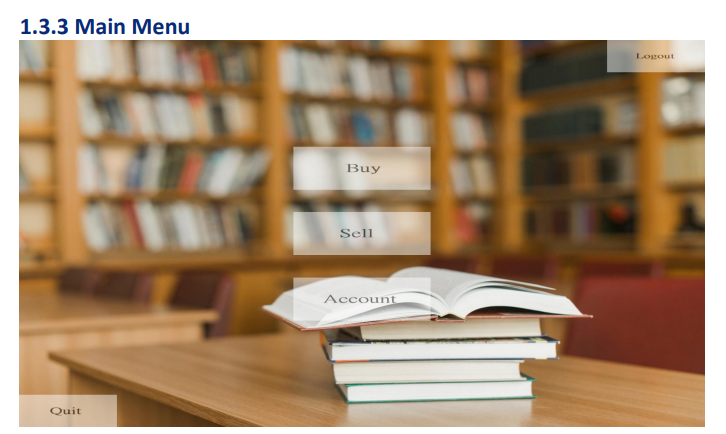
\includegraphics[width=0.9\textwidth]{proj1.png}
        \caption{ICT SBA}
    \end{minipage}\hfill
    \begin{minipage}{0.3\textwidth}
        \centering
        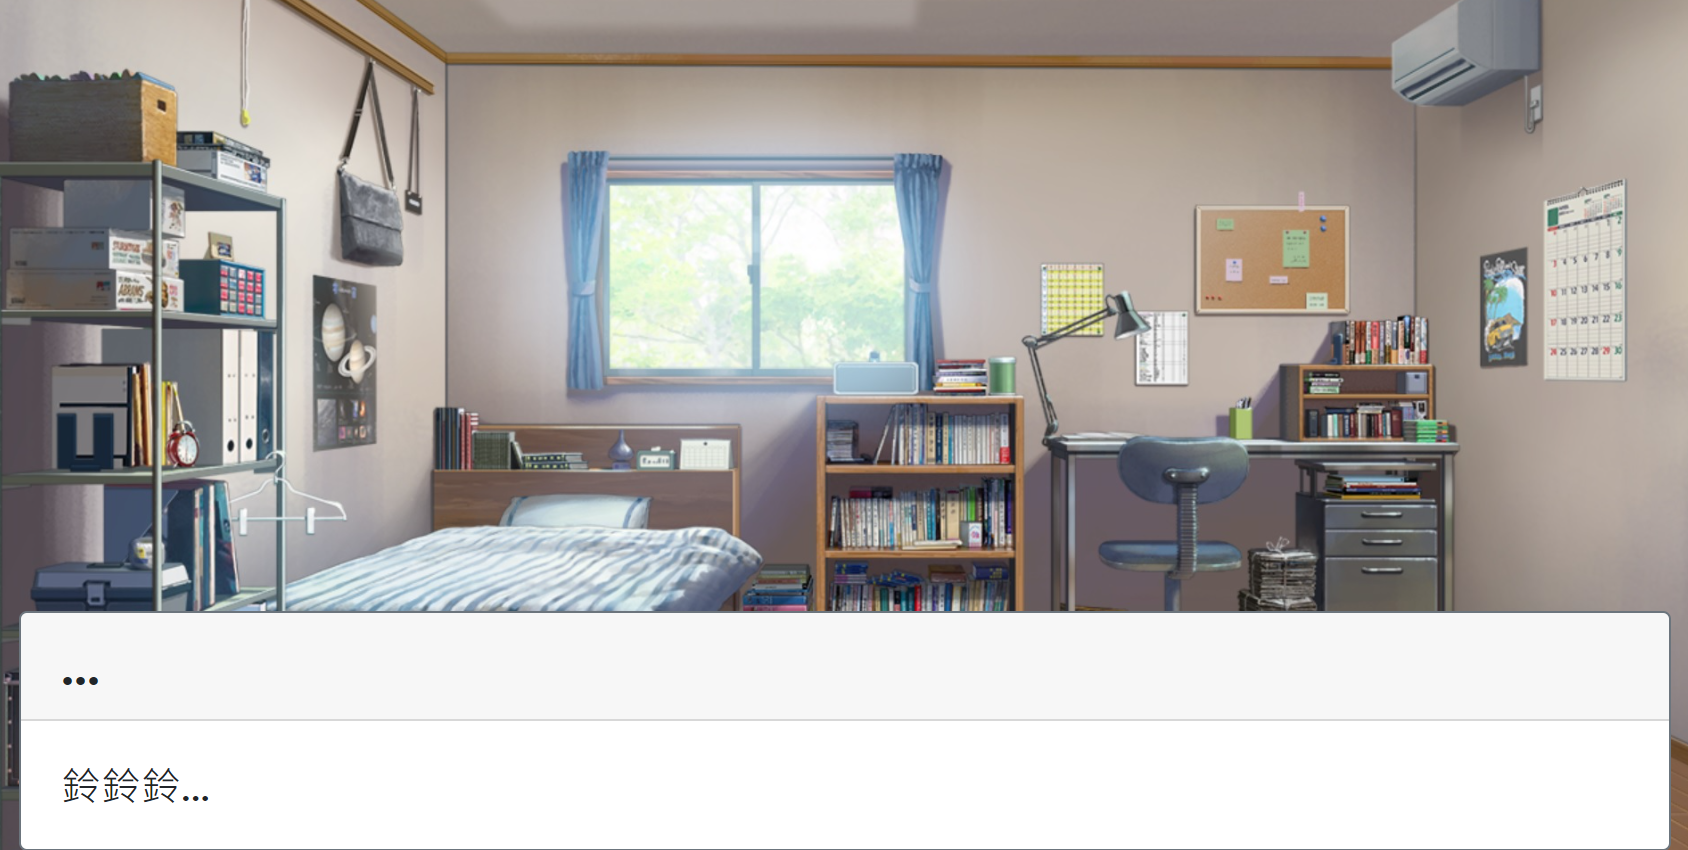
\includegraphics[width=0.9\textwidth]{proj2.png}
        \caption{visual novel}
    \end{minipage}\hfill
    \begin{minipage}{0.3\textwidth}
        \centering
        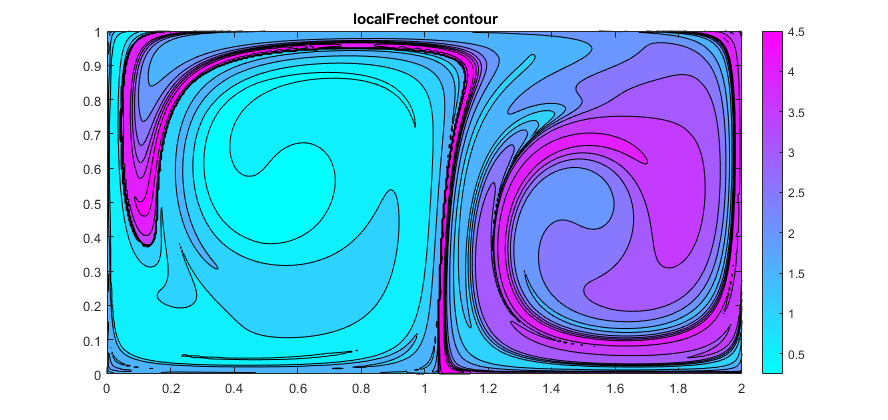
\includegraphics[width=0.9\textwidth]{proj3.png}
        \caption{computation}
    \end{minipage}
  \end{figure}
\end{frame}

\begin{frame}{What do you expect to learn here?}
  \begin{itemize}
    \item Basic syntax of Python
    \item Ability of read and write program in a structured way
    \item Problem Solving skills
    \item Mathematics skills
    \item \sout{Debug and suffer}
  \end{itemize}
\end{frame}

\begin{frame}{What will you need to do?}
  \begin{itemize}
    \item In-class practice
    \item Small and simple group homework problem (to be assigned next lesson)
  \end{itemize}
\end{frame}

\begin{frame}{What are expected from you?}
  \begin{block}{1. Practice and be patient}
    Work on exercise problems yourselves or with your friends and do coding hands-on; Coding can sometimes be frustrating, but don't give up too easily!
  \end{block}
\end{frame}
\begin{frame}{What are expected from you?}
  \begin{block}{2. Speak out}
    Speak out if you don't understand or you got any ideas to share. There's no shame in asking questions. Discuss with others and share your ideas / difficultites! Also feel free to contact me if you have any thing related to programming that you want me to include in the lesson.
  \end{block}
\end{frame}
\begin{frame}{What are expected from you?}
  \begin{block}{3. Explore}
    I will be teaching you for only 8 lessons, it is impossible to cover all the interesting material in the world of coding and programming, besides suggesting material for me to include in the lecture, you can (and also suggested to) explore yourself in the internet and try out different interesting projects.
  \end{block}
\end{frame}

\begin{frame}{Some Extra infomation}
    \begin{itemize}
      \item Course website: \href{https://www.stmc.edu.hk/codingteam/}{https://www.stmc.edu.hk/codingteam/}
      \item Whatsapp Group: \href{https://chat.whatsapp.com/JPaKBmGSyyp0cLDNDjqePJ}{https://chat.whatsapp.com/JPaKBmGSyyp0cLDNDjqePJ}
    \end{itemize}
    \begin{figure}[h!]
      \centering
      
\includegraphics[width=0.25\textwidth]{WhatsappGrpURL.png}
      \caption{Whatsapp Group}
    \end{figure}
\end{frame}

\begin{frame}{Without further ado, Let's get started ...}
  
\end{frame}

\end{document}
